% ----------------------------------------------------------

% ----------------------------------------------------------
\chapter{Desenvolvimento do Trabalho}

% ----------------------------------------------------------
\subsection{Requisitos}
\subsubsection{Lista de requisitos}
Segue os requisitos do projeto
% ----------------------------------------------------------
\begin{table}[htb]
	\centering
	\caption{\label{Formatação do texto.}Requisitos funcionais}
	\begin{tabular}{|l|p{11cm}|}
	\hline
	\textbf{Identificação} & \textbf{Requisito}\\ \hline
	RF01 & Manter usuário \\ \hline
	RF02 & Realizar login \\ \hline
	RF03 & Cadastro de anúncio \\ \hline
	RF04 & Avaliação do profissional\\ \hline
	RF05 & Histórico de serviços prestados \\ \hline
	RF06 & Histórico de serviços contratados \\ \hline
	RF07 & Candidatar no anúncio \\ \hline
	RF08 & Concluir anúncio \\ \hline
	\end{tabular}
	\fonte{\textcite{Elaborado pelos autores(2023)}.}
\end{table}

\begin{table}[htb]
	\centering
	\caption{\label{Formatação do texto.}Requisitos não funcionais}
	\begin{tabular}{|l|p{11cm}|}
	\hline
	\textbf{Identificação}    & \textbf{Requisito}\\ \hline
	RNF01        			  & Banco de dados relacional(PostgreSQL)\\ \hline
	RNF02        			  & Interface mobile em ReactJS Native\\ \hline
	\end{tabular}
	\fonte{\textcite{Elaborado pelos autores(2023)}.}
\end{table}

\subsubsection{ Lista de Regras de Negócio}
Segue a tabela com as regras de negócio do sistema.
\clearpage
\begin{table}[htb]
	\centering
	\caption{\label{Formatação do texto.}Lista de Regras de Negócio}
	\begin{tabular}{|l|p{8cm}|p{3cm}|}
		\hline
		\textbf{Identificação} & \textbf{Regras de Negócio} & \textbf{Requisito associado} \\ \hline
		RN01 & Validação CPF válido e único. & RF1 \\ \hline
		RN02 & RValidação de email válido e único. & RF02 \\ \hline
		RN03 & O prestador de serviço NÃO poderá se candidatar para, realizar um serviço caso tenha um serviço marcado para a mesma data e hora. & RF07 \\ \hline
		RN04 & O cliente só poderá selecionar um profissional, para realizar o serviço. & RF08 \\ \hline
		RN05 & O cliente só poderá avaliar um profissional após a conclusão do serviço. & RF08, RF04 \\ \hline
		RN06 & O prestador de serviços só poderá ver e se candidatar para serviços relacionados com o seu perfil  & RF07 \\ \hline
		RN07 & O cliente não poderá fazer um anúncio com a data do passado  & RF03 \\ \hline
		RN08 & Caso o anúncio tenha uma data de expiração ele não deverá aparecer em tela e o anunciante deverá ser notificado & RF03 \\ \hline
	\end{tabular}
	\fonte{\textcite{Elaborado pelos autores(2023)}.}
\end{table}


\subsubsection{ Descrição dos requisistos}
\clearpage
\begin{table}[htb]
	\centering
	\caption{\label{Formatação do texto.}Descrição RF01}	
	\begin{tabular}{|l|p{11cm}|}
		\hline
		\textbf{Incremento}    & Iteração 03\\ \hline
		\textbf{Nome}    & Manter usuário\\ \hline
		\textbf{Tipo}    & Funcional\\ \hline
		\multicolumn{2}{|c|}{Descrição}\\ \hline
		\multicolumn{2}{|p{12cm}|}{
			O sistema deve permitir o cadastro de usuários e o gerenciamento de suas informações. \newline
			\newline Critérios de Aceitação: \newline
			O sistema deve permitir o cadastro de novos clientes com as informações básicas (nome, e-mail, senha, CPF, cidade, endereço e telefone); \newline
			\newline O sistema deve permitir o cadastro de novos prestadores com as informações básicas (nome, e-mail, senha, CPF, ou CNPJ, cidade, categoria do serviços prestados e telefone); \newline
			\newline O sistema deve permitir a atualização das informações do usuário, incluindo nome, e-mail e senha; \newline
			\newline O sistema deve permitir a exclusão do usuário; \newline
			O sistema deve garantir a segurança das informações dos usuários, armazenando as senhas de forma criptografada.
			} \\ \hline
	\end{tabular}
	\fonte{\textcite{Elaborado pelos autores(2023)}.}
\end{table}

\subsubsection{ Prototipação do caso de uso Manter Usuário}
	Segue a baixo a prototipação do requisito RF01.
\begin{figure}[hbb]
	\caption{Tela de cadastro - Passo 1}
	\begin{center}
		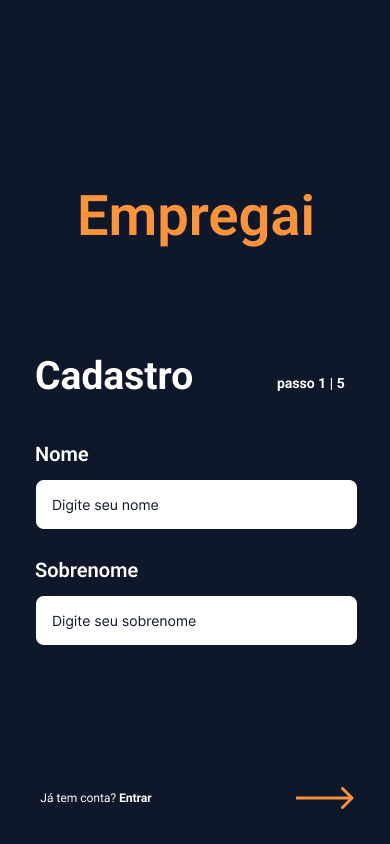
\includegraphics[width=0.3\textwidth]{images/Cadastro-1.png}
	\end{center}
	\fonte{Elaborado pelos autores(2023)}
	No primeiro passo o usuário deverá informa seu nome e o sobrenome
\end{figure}

\begin{figure}[hbb]
	\caption{Tela de cadastro - Passo 2}
	\begin{center}
		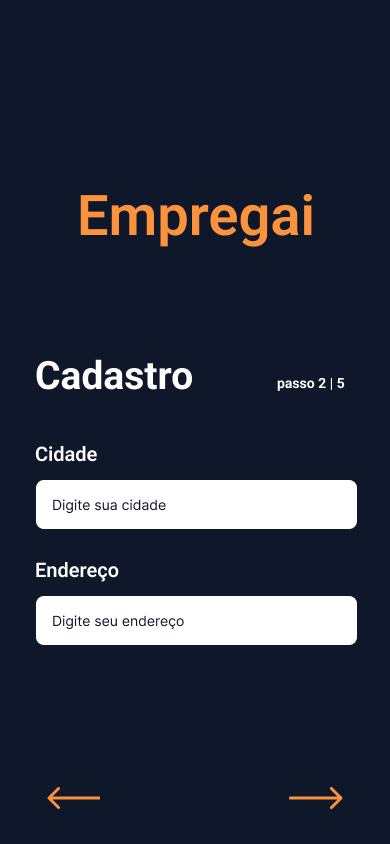
\includegraphics[width=0.3\textwidth]{images/Cadastro-2.png}
	\end{center}
	\fonte{Elaborado pelos autores(2023)}
	No segundo passo o usuário deverá informa a cidade e o endereço
\end{figure}

\begin{figure}[hbb]
	\caption{Tela de cadastro - Passo 3}
	\begin{center}
		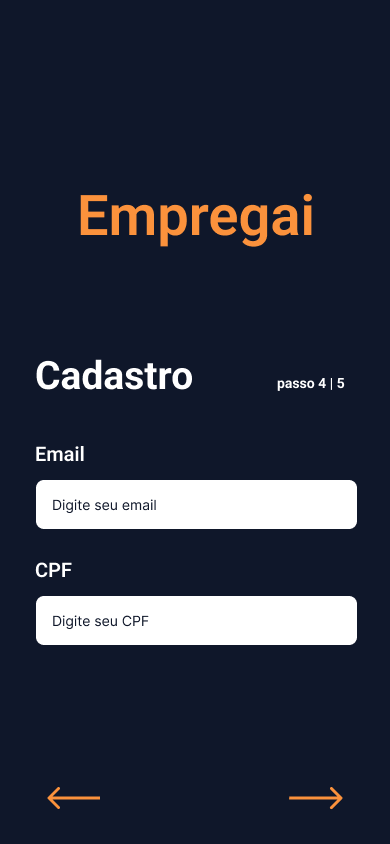
\includegraphics[width=0.3\textwidth]{images/Cadastro-4.png}
	\end{center}
	\fonte{Elaborado pelos autores(2023)}
	No terceiro passo o usuário deverá informa seu email e o CPF
\end{figure}

\begin{figure}[hbb]
	\caption{Tela de cadastro - Passo 4}
	\begin{center}
		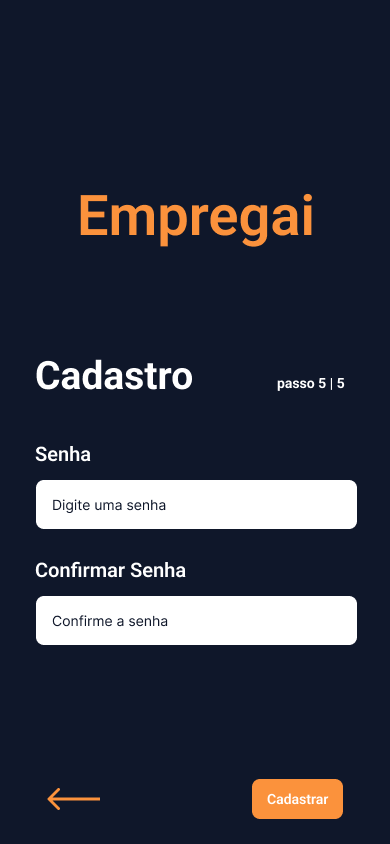
\includegraphics[width=0.3\textwidth]{images/Cadastro-5.png}
	\end{center}
	\fonte{Elaborado pelos autores(2023)}
	No quarto passo o usuário deverá informa uma senha.
\end{figure}
\clearpage
\begin{table}[htb]
	\centering
	\caption{\label{Formatação do texto.}Descrição RF02}	
	\begin{tabular}{|l|p{11cm}|}
		\hline
		\textbf{Incremento}    & Iteração 03\\ \hline
		\textbf{Nome}    & Realizar login\\ \hline
		\textbf{Tipo}    & Funcional\\ \hline
		\multicolumn{2}{|c|}{Descrição}\\ \hline
		\multicolumn{2}{|p{12cm}|}{
			O sistema deve permitir que os usuários realizem login para acessar suas contas. \newline
			\newline Critérios de Aceitação: \newline
			O sistema deve apresentar um formulário de login com os campos de e-mail e senha; \newline
			\newline O sistema deve validar as informações de login e permitir o acesso ao usuário caso as informações estejam corretas;\newline
			\newline O sistema deve apresentar uma mensagem de erro caso as informações de login estejam incorretas;
			}\\ \hline
	\end{tabular}
	\fonte{\textcite{Elaborado pelos autores(2023)}.}
\end{table}

\clearpage
\begin{figure}[htb]
	\caption{Tela de login}
	\begin{center}
		
\includegraphics[width=0.3\textwidth]{images/RF02.png}
	\end{center}
	\fonte{Elaborado pelos autores(2023)}
\end{figure}

\clearpage
\begin{table}[htb]
	\centering
	\caption{\label{Formatação do texto.}Descrição RF03}	
	\begin{tabular}{|l|p{11cm}|}
		\hline
		\textbf{Incremento}    & Iteração 04\\ \hline
		\textbf{Nome}    & Cadastro de anúncio\\ \hline
		\textbf{Tipo}    & Funcional\\ \hline
		\multicolumn{2}{|c|}{Descrição}\\ \hline
		\multicolumn{2}{|p{12cm}|}{
			O sistema deve permitir que os clientes cadastrem seus anúncios de serviços. \newline
			\newline Critérios de Aceitação: \newline
			O sistema deve apresentar um formulário para o cadastro de anúncio, contendo informações como título, descrição, categoria eu localização; \newline
			\newline O sistema deve permitir que o cliente edite e exclua seus anúncios;\newline
			\newline O sistema deve validar as informações inseridas pelo cliente, garantindo que o anúncio contenha informações suficientes e válidas para ser publicado.
			} \\ \hline
	\end{tabular}
	\fonte{\textcite{Elaborado pelos autores(2023)}.}
\end{table}

\clearpage
\begin{table}[htb]
	\centering
	\caption{\label{Formatação do texto.}Descrição RF07}	
	\begin{tabular}{|l|p{11cm}|}
		\hline
		\textbf{Incremento}    & Iteração 04\\ \hline
		\textbf{Nome}    & Candidatar no anúncio\\ \hline
		\textbf{Tipo}    & Funcional\\ \hline
		\multicolumn{2}{|c|}{Descrição}\\ \hline
		\multicolumn{2}{|p{12cm}|}{
			O sistema deve permitir que prestadores de serviços possam se candidatar a anúncios criados pelos clientes. \newline
			\newline Critérios de Aceitação: \newline
			O prestador de serviços deve ser capaz de visualizar os anúncios disponíveis para candidatura; \newline
            O prestador de serviços deve poder se candidatar a um anúncio ao clicar em um botão específico; \newline
			O cliente deve ser notificado da candidatura do prestador de serviços; \newline
			O cliente deve ser capaz de visualizar as candidaturas recebidas para seu anúncio; \newline
			O cliente deve ser capaz de selecionar e contatar o prestador de serviços escolhido para o anúncio.
			} \\ \hline
	\end{tabular}
	\fonte{\textcite{Elaborado pelos autores(2023)}.}
\end{table}

\clearpage
\begin{table}[htb]
	\centering
	\caption{\label{Formatação do texto.}Descrição RF08}	
	\begin{tabular}{|l|p{11cm}|}
		\hline
		\textbf{Incremento}    & Iteração 05\\ \hline
		\textbf{Nome}    & Concluir o anúncio\\ \hline
		\textbf{Tipo}    & Funcional\\ \hline
		\multicolumn{2}{|c|}{Descrição}\\ \hline
		\multicolumn{2}{|p{12cm}|}{
			O sistema deve permitir que clientes concluam um anúncio após a seleção de um prestador de serviços. \newline
			\newline Critérios de Aceitação: \newline
			O cliente deve ser capaz de visualizar a lista de candidaturas recebidas para o anúncio; \newline
            O cliente deve ser capaz de selecionar um prestador de serviços para realizar o trabalho; \newline
			O cliente deve ser capaz de confirmar a seleção do prestador de serviços; \newline
			O prestador de serviço de se informado que sua candidatura foi aceita; \newline
			O sistema deve permitir que o cliente avalie o prestador de serviços após a conclusão do trabalho.
			} \\ \hline
	\end{tabular}
	\fonte{\textcite{Elaborado pelos autores(2023)}.}
\end{table}

\clearpage
\begin{table}[htb]
	\centering
	\caption{\label{Formatação do texto.}Descrição RF04}	
	\begin{tabular}{|l|p{11cm}|}
		\hline
		\textbf{Incremento}    & Iteração 06\\ \hline
		\textbf{Nome}    & Avaliação do profissional\\ \hline
		\textbf{Tipo}    & Funcional\\ \hline
		\multicolumn{2}{|c|}{Descrição}\\ \hline
		\multicolumn{2}{|p{12cm}|}{
			O sistema deve permitir que os clientes avaliem os prestadores de serviço após a realização do serviço. \newline
			\newline Critérios de Aceitação: \newline
			O sistema deve apresentar um campo de avaliação com uma escala numérica ou de estrelas e um campo para o cliente deixar um comentário sobre a qualidade do serviço prestado; \newline
			\newline O sistema deve permitir que o cliente avalie apenas os prestadores de serviço que já foram contratados por ele; \newline
			\newline O sistema deve disponibilizar as avaliações dos prestadores de serviço para que outros clientes possam consultar antes de contratar os serviços dos mesmos.
			} \\ \hline
	\end{tabular}
	\fonte{\textcite{Elaborado pelos autores(2023)}.}
\end{table}

\clearpage
\begin{table}[htb]
	\centering
	\caption{\label{Formatação do texto.}Descrição RF05}	
	\begin{tabular}{|l|p{11cm}|}
		\hline
		\textbf{Incremento}    & Iteração 07\\ \hline
		\textbf{Nome}    & Histórico de serviços prestados\\ \hline
		\textbf{Tipo}    & Funcional\\ \hline
		\multicolumn{2}{|c|}{Descrição}\\ \hline
		\multicolumn{2}{|p{12cm}|}{
			O sistema deve permitir que os prestadores de serviço visualizem seu histórico de serviços prestados. \newline
			\newline Critérios de Aceitação: \newline
			O sistema deve exibir uma lista de todos os serviços prestados pelo prestador, com informações como o título do anúncio e a data de realização; \newline
			\newline O sistema deve permitir que o cliente avalie apenas os prestadores de serviço que já foram contratados por ele; \newline
			\newline O sistema deve disponibilizar as avaliações dos prestadores de serviço para que outros clientes possam consultar antes de contratar os serviços dos mesmos.
			} \\ \hline
	\end{tabular}
	\fonte{\textcite{Elaborado pelos autores(2023)}.}
\end{table}

\clearpage
\begin{table}[htb]
	\centering
	\caption{\label{Formatação do texto.}Descrição RF06}	
	\begin{tabular}{|l|p{11cm}|}
		\hline
		\textbf{Incremento}    & Iteração 07\\ \hline
		\textbf{Nome}    & Histórico de serviços contratados\\ \hline
		\textbf{Tipo}    & Funcional\\ \hline
		\multicolumn{2}{|c|}{Descrição}\\ \hline
		\multicolumn{2}{|p{12cm}|}{
			O sistema deve permitir que o cliente tenha acesso ao histórico de serviços contratados por ele, incluindo informações como data, valor, nome do prestador de serviço e avaliação. \newline
			\newline Critérios de Aceitação: \newline
			O sistema deve apresentar uma lista dos serviços contratados pelo cliente; \newline
            Cada serviço deve apresentar informações como data, nome do prestador de serviço e avaliação; \newline
			\newline O histórico deve ser atualizado automaticamente após a conclusão do serviço;
			} \\ \hline
	\end{tabular}
	\fonte{\textcite{Elaborado pelos autores(2023)}.}
\end{table}


\clearpage
\begin{table}[htb]
	\centering
	\caption{\label{Formatação do texto.}Descrição RNF01}	
	\begin{tabular}{|l|p{11cm}|}
		\hline
		\textbf{Nome}    & Banco de dados relacional(PostgreSQL)\\ \hline
		\textbf{Tipo}    & Não funcional\\ \hline
		\multicolumn{2}{|c|}{Descrição}\\ \hline
		\multicolumn{2}{|p{12cm}|}{
			O sistema deve utilizar um banco de dados relacional PostgreSQL para armazenamento de dados. \newline
			\newline Critérios de Aceitação: \newline
			O banco de dados deve ser implementado em PostgreSQL;
			Deve ser garantida a integridade e consistência dos dados armazenados;\newline
			\newline O esquema do banco de dados deve ser projetado de acordo com as necessidades do sistema; \newline
			\newline O acesso ao banco de dados deve ser realizado através de um usuário com permissões adequadas; \newline
			\newline O sistema deve permitir a exclusão do usuário; \newline
			O banco de dados deve ser capaz de suportar um grande volume de dados e garantir a disponibilidade do sistema.
			} \\ \hline
	\end{tabular}
	\fonte{\textcite{Elaborado pelos autores(2023)}.}
\end{table}

\clearpage
\begin{table}[htb]
	\centering
	\caption{\label{Formatação do texto.}Descrição RNF02}	
	\begin{tabular}{|l|p{11cm}|}
		\hline
		\textbf{Nome}    & Interface mobile em ReactJS Native utilizando Expo\\ \hline
		\textbf{Tipo}    & Não funcional\\ \hline
		\multicolumn{2}{|c|}{Descrição}\\ \hline
		\multicolumn{2}{|p{12cm}|}{
			O sistema deve utilizar React Native em conjunto com a plataforma Expo para desenvolvimento da interface mobile. \newline
			\newline Critérios de Aceitação: \newline
			A interface deve ser desenvolvida em React Native utilizando a plataforma Expo; \newline
			\newline A interface deve ser responsiva e adaptável a diferentes tamanhos de tela;\newline
			\newline A interface deve ser desenvolvida de acordo com as diretrizes da plataforma para garantir compatibilidade e desempenho.
			} \\ \hline
	\end{tabular}
	\fonte{\textcite{Elaborado pelos autores(2023)}.}
\end{table}